\section{Architecture}

Diogenes has three main components:
an honesty checker for \coco,
an honesty checker for Java,
and an Eclipse plugin which integrates the two analyses
with an editor of \coco.
We illustrate the architecture of our tools in~\Cref{fig:architecture}.

The \coco honesty checker implements the  
verification technique introduced in~\cite{BCPZ15jlamp}.
This technique is built upon an alternative semantics of \coco 
which abstracts both values (sent, received, and in conditional expressions) 
and the actual \emph{context} wherein a process is executed.
This abstraction is a \emph{sound} over-approximation of honesty:
namely, if the abstraction of a process is honest,
then also the concrete one is honest.
Further, in the fragment of \coco without conditional statements
the analysis is also \emph{complete},
\ie if a concrete process is honest, then also its abstraction is honest.
For processes without delimitation/parallel under process definitions,
the associate abstraction is finite-state, 
hence we can verify their honesty by model checking a (finite) state space.
Our implementation 
first translates a \coco process into a Maude term~\cite{Maude01}, 
and then uses the Maude LTL model checker~\cite{Eker02maude}
to decide honesty of its abstract semantics.

%\paragraph{Diogenes.}
The Java honesty checker is developed on top of \emph{Java PathFinder}
(JPF, \cite{lerda2001addressing,visser2003model}).
The JPF core is a Virtual Machine for Java bytecode
that can be configured to act as a model-checker.
It provides the concept of \emph{execution choice}
and \emph{state backtracking}, allowing multiple state exploration.
%
We exploit its capabilities in order to extract a \coco model
from a Java program. We implement a \emph{listener} that allow us
to catch specific method invocations representing I/O actions
directed to the middleware~\cite{CO2middleware},
and simulate \emph{all} the possible response that 
the application can receive from it.
Once the \coco model is extracted, we verify its honesty
with the model checking technique of~\cite{BCPZ15jlamp}.
Therefore, the analysis strongly depends on the Maude model-checker,
as shown by the data-flow in \Cref{fig:architecture}.
\bartnote{+ commento sulla tecnica di analisi: ad esempio, sotto quali ipotesi e' corretta?}

The Eclipse plugin \bartnote{dire prima cosa fa, e poi dare qualche insight}
% On the contrary, the Eclipse plugin has no dependencies, and
% it integrates the possibility to directly call 
% the Maude model-checker, reporting its output into the Eclipse console.
%
The plugin relies on
Xtext~\cite{xtext-site}, a framework for developing programming languages, 
and Xsemantics~\cite{xsemantics-site}, a domain-specific language for writing type systems
for Xtext-based languages.
%
We use Xtext to define the grammar of \coco.
\bartnote{giusto? si usa per altre cose? c'e' da dire altre cose interessanti sul plugin? mi sembra che questa parte andrebbe espanda un poco}
% We implement an Xtext grammar focusing on~\cite{BCPZ15jlamp},
% and we extend it in order to allow a complete mapping between \coco and Java.


\begin{figure}[t]
    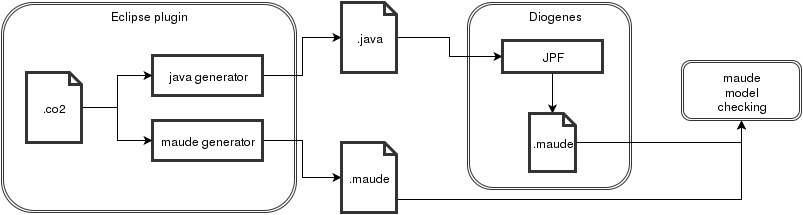
\includegraphics[width=\textwidth]{img/diogenes-arch.png}
    \caption{Data flow schema}
    \label{fig:architecture}
\end{figure}